\chapter{Introducción a Numpy\\ Introduction to Numpy}\index{Numpy} \index[eng]{Numpy}
\epigraph{When the going gets tough, the tough get going}{Popular Witticism (US)}
\begin{paracol}{2}
\section{Numpy: un paquete de Python para cálculo nu\-mérico}
En el capítulo \ref{ch:intpr}, vimos cómo importar mó\-dulos de python en un script o directamente en el terminal de Ipython, de modo que podamos reutilizar el código contenido en ellos. Numpy es un libraría de python que contiene funciones y variables específicamente diseñadas para el cálculo numérico. Está estructurada en forma de módulos y submódulos de modo que para utilizarla en nuestros programas basta  importarla en nuestros script, importar sus submodulos o importar sus funciones.
La base de Numpy la constituyen objetos y operaciones algebráicas. En esta sección vamos a repasar algunos conceptos fundamentales de  álgebra lineal y cómo pueden manejarse empleando Python. No daremos definiciones precisas ni tampoco demostraciones, ya que tanto unas como otras se verán en detalle en la asignatura de álgebra.

\paragraph{matrices.} Desde un punto de vista funcional definiremos una matriz como una tabla bidimensional de números ordenados en filas y columnas,

\end{paracol}

\begin{equation*}
A=
\begin{pmatrix}
1& \sqrt{2}& 3.5& 0\\
-2& \pi& -4.6& 4\\
7& -19& 2.8& 0.6
\end{pmatrix}
\end{equation*}

\begin{paracol}{2}
Cada línea horizontal de números constituye una \emph{fila} de la matriz y cada línea horizontal una \emph{columna} de la misma.

A una matriz con $m$ filas y $n$ columnas se la denomina matriz de orden $m\times n$. $m$ y $n$ son la dimensiones de la matriz y se dan siempre en el mismo orden: primero el número de filas y después el de columnas. Así, la matriz $A$ del ejemplo anterior es una matriz $3\times 4$, y como esta formada por números reales se dice que $A\in\mathbb{R}^{3\times 4}$. El orden de una matriz expresa el tamaño de la matriz.

Dos matrices son iguales si tienen el mismo orden, y los elementos que ocupan en ambas matrices los mismo lugares son iguales.

Una matriz es cuadrada, si tiene el mismo número de filas que de columnas. Es decir es de orden $n\times n$.

Mientras no se diga expresamente lo contrario, emplearemos letras mayúsculas $A, B, \cdots$ para representar matrices. La expresión $A_{m\times n}$ indica que la matriz $A$ tiene dimensiones $m \times n$. Para denotar los elementos de una matriz, emplearemos la misma letra en minúsculas empleada para nombrar la matriz, indicando mediante subíndices, y siempre por este orden, la fila y la columna a la que pertenece el elemento. Así por ejemplo $a_{ij}$ representa al elemento de la matriz $A$, que ocupa la fila $i$ y la columna $j$.
\end{paracol}
\begin{equation*}
A=
\begin{pmatrix}
1& \sqrt{2}& 3.5& 0\\
-2& \pi& -4.6& 4\\
7& -19& 2.8& 0.6
\end{pmatrix}
\rightarrow a_{23}=-4.6
\end{equation*}
\begin{paracol}{2}
\paragraph{vectores}
A una matriz compuesta por una sola fila, la denominaremos vector fila. A una matriz compuesta por una sola columna la denominaremos vector columna. Siempre que hablemos de un vector, sin especificar más, entenderemos que se trata de un vector columna.\footnote{Esta identificación de los vectores como vectores columna no es general. La introducimos porque simplifica las explicaciones posteriores.} Para representar vectores, emplearemos letras minúsculas. Para representar sus elementos añadiremos a la letra que representa al vector un subíndice indicando la fila a la que pertenece el elemento.
\end{paracol}
\begin{equation*}
a=
\begin{pmatrix}
a_1\\
a_2\\
\vdots \\
a_i\\
\vdots \\
a_n
\end{pmatrix}
\end{equation*}
\begin{paracol}{2}
Podemos asociar los puntos del plano con los vectores de dimensión dos. Para ello, usamos una representación cartesiana, en la que los elementos del vector son los valores de las coordenadas $(x,y)$ del punto del plano que representan. Cada vector se representa gráficamente mediante una flecha que parte del origen de coordenadas y termina en el punto $(x,y)$ representado por el vector. La figura \ref{fig:vectores} representa los vectores,
\end{paracol}
\begin{equation*}
a=
\begin{pmatrix}
1\\
2
\end{pmatrix},
b=
\begin{pmatrix}
2\\
-3
\end{pmatrix},
c=
\begin{pmatrix}
0\\
-2
\end{pmatrix}
\end{equation*}


\begin{figure}[h]
\centering
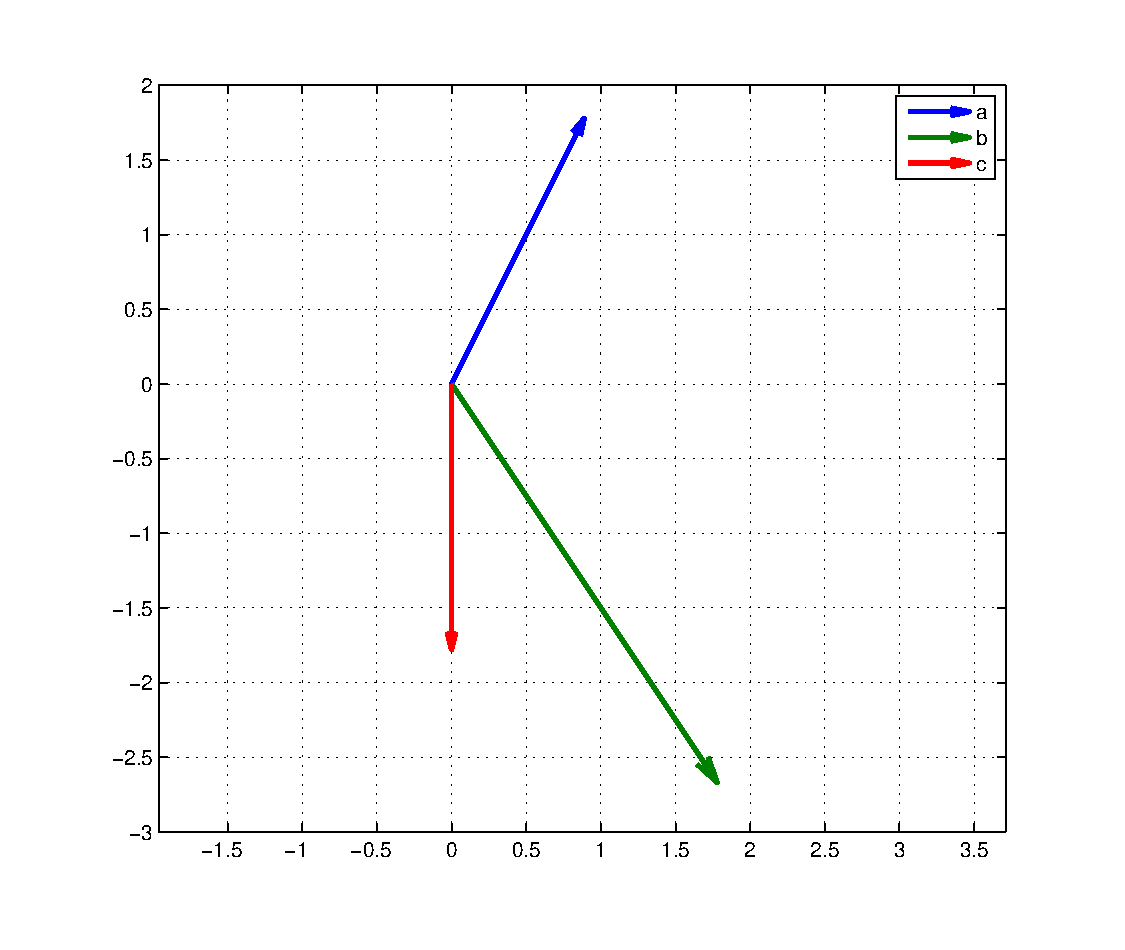
\includegraphics[width=7cm]{vectores.eps}
\caption{Representación gráfica de vectores en el plano}
\label{fig:vectores}
\end{figure}

\begin{paracol}{2}
\subsection{Vectores y matrices en\\ Numpy.} \index{Vectores!en Numpy} \index{Matrices!en Numpy} 
\paragraph{Matrices.} Una de las característica más interesantes de Numpy, es la posibilidad de crear fácilmente matrices. Se pueden crear de diferentes maneras, la más elemental de todas ellas, emplea la funcion de Numpy \mintinline{python}{array} aplicada a una lista de filas de la matriz que se quiere construir. Cada fila debe ser a su vez una lista de números. Evidentemente, para que se pueda construir la matriz, todas las filas deben tener el mismo número de elementos. El siguiente ejemplo muestra como construir una matriz de dos filas y tres columnas,
\end{paracol}

\begin{center}
    \begin{minipage}{0.4\textwidth}
    \begin{minted}{python}
In [3]: import numpy as np

In [4]: A = np.array([[1,2,3],[4,5,6]])

In [5]: print(A)
[[1 2 3]
 [4 5 6]]

In [6]: L = [[1,2,3],[4,5,6]]

In [7]: B = np.array(L)

In [9]: print(L)
[[1, 2, 3], [4, 5, 6]]

In [10]: print(B)
[[1 2 3]
 [4 5 6]]
 \end{minted}
\end{minipage}
 \end{center}
\begin{paracol}{2} 
Lo primero que hacemos es importar Numpy, lo importamos usando como alias la abreviatura np, porque es más cómodo a la hora de llamar a funciones específicas de Numpy.  Hemmos construido dos matrices iguales \mintinline{python}{A} y \mintinline{python}{B}. En el primer caso hemos creado directamente dentro de la llamada a la función \mintinline{python}{array}, la lista a partir de la cual construimos la matriz. En el segundo caso, hemos construido primero una lista \mintinline{python}{L}, y luego hemos empleado dicha lista como variable de entrada de la función \mintinline{python}{array}. Si nos fijamos en las líneas [9] y [10], vemos como Python distingue la lista ---todos sus elementos aparacen representados en la misma línea---, de la matriz en la que cada fila ocupa una línea distinta. Podemos construir matrces a partir de listas y variables ya definidas, siempre que seamos coherentes con el criterio de que cada fila se cree a partir de una lista y que todas las filas tengan los mismos elementos,
\end{paracol}
\begin{center}
    \begin{minipage}{0.4\textwidth}
        \begin{minted}{python}
In [23]: a =1; b= 2; c =3

In [24]: d =[4,5,6]

In [25]: C = np.array([[a,b,c],d])

In [26]: print(C)
[[1 2 3]
 [4 5 6]]

In [27]: C = np.array([[a,b,c],d,[7,8,9]])

In [28]: print(C)
[[1 2 3]
 [4 5 6]
 [7 8 9]]
        \end{minted}
    \end{minipage}
\end{center}
\begin{paracol}{2}
\paragraph*{Indexación.} \index{Numpy!indexación}Al igual que se hace en álgebra, Numpy es capaz de referirse a un elemento cualquiera de una matriz empleando índices para determinar su posición (fila y columna) dentro de la matriz.
\end{paracol}
\begin{equation*}
A=
\begin{pmatrix}
a_{11}&a_{12}&a_{13}\\
a_{21}&a_{22}&a_{23}\\
a_{31}&a_{32}&a_{33}
\end{pmatrix}
\end{equation*}

\begin{paracol}{2}
Sin embargo,  criterio para referirse a un elemento concreto de una matriz, en Numpy está heredado de las listas: se indica el nombre de la variable que contiene la matriz y a continuación, entre corchetes y separados por una coma, el índice de su fila y después él de su columna \textbf{pero empezando a contar desde $0$}. Es decir, la primera fila de una matriz de dimensión $m\times n$ es la fila $0$ y la última es la fila $m-1$. De modo análogo su primera columna es la $0$ y su última columna es la $n-1$,    
\end{paracol}
\begin{center}
    \begin{minipage}{0.3\textwidth}
        \begin{minted}{python}
In [31]: print(C)
[[1 2 3]
 [4 5 6]
 [7 8 9]]

In [32]: C[1,2]
Out[32]: 6

In [33]: C[0,0]
Out[33]: 1
        \end{minted}
    \end{minipage}
\end{center}

\begin{paracol}{2}
Numpy puede seleccionar dentro de una matriz no solo elementos aislados, sino también submatrices completas. 
Para ello, emplea un símbolo reservado, el símbolo \emph{dos puntos} $:$. Este símbolo se emplea para recorrer valores desde un valor inicial hasta un valor final, con un incremento o paso fijo. La sintaxis es: \mintinline{python}{inicio:fin:paso}, Es importante tener en cuenta que Numpy detendrá la cuenta en el valor \mintinline{python}{paso-1}. Además, si no indicamos el tamaño del paso, Numpy tomará por defecto un paso igual a uno. En este caso basta emplear un único símbolo \emph{dos puntos} para separar el valor de inicio del valor final,
\end{paracol}

\begin{center}
        \begin{minted}{python}
In [87]: D = numpy.array([[1.,2.,3.],[4.,5.,6.],[-2,-3,0],[3,2,1]])

In [88]: print(D)
[[ 1.  2.  3.]
 [ 4.  5.  6.]
 [-2. -3.  0.]
 [ 3.  2.  1.]]

In [90]: D[0:1,0:3]
Out[90]: array([[1., 2., 3.]])

In [91]: D[0:2,0:2]
Out[91]: 
array([[1., 2.],
       [4., 5.]])

In [92]: D[2:3,1:2]
Out[92]: array([[-3.]])

In [93]: D[3:4,0:3]
Out[93]: array([[3., 2., 1.]])

In [94]: D[0:4,0:3]
Out[94]: 
array([[ 1.,  2.,  3.],
       [ 4.,  5.,  6.],
       [-2., -3.,  0.],
       [ 3.,  2.,  1.]])

In [95]: D[0:4,2:3]
Out[95]: 
array([[3.],
       [6.],
       [0.],
       [1.]])
       \end{minted}
\end{center}

\begin{paracol}{2}
La línea [90], extrae un vector fila con los elementos de la primera fila de la matriz \mintinline{python}{D}. La fila [91] extrae una matriz de dimension $2\times 2$ con los cuatro elementos de la esquina superior izquierda de la matriz original. La fila [92] extrae un único elemento pero sigue siendo una matriz de dimensión $1 \times 1$, por tanto es distinto que si empleamos la indexación directa del elemento: \mintinline{python}{D[2,1]}. La línea [93] nos devuelve un vector fila con la última fila de la matriz. La línea [94], nos devuelve de nuevo la matriz entera. Por último la línea 95 nos devuelve un vector columna con la primera columna de la matriz.

Hemos dicho que la línea [94] nos devuelve un vector columna. Bueno, sí y no; vamos a verlo más despacio.

\paragraph{Vectores.}
Cuando introducimos los vectores, distinguimos entre vectores filas y columna, definiéndolos como matrices de una sola fila o una sola columna. Sin embargo, en Numpy, se sigue un criterio distinto que permite generalizar el concepto de matriz asociándolo con el de tensor. Sin entrar en detalles\footnote{Una definición formal del concepto de tensor, queda fuera del alcance de estos apuntes}, podemos decir que un tensor es un objeto algebráico caracterizado por dos parámetros el orden y la dimensión. Así un escalar $a \in \mathbb{R}$ es un tensor de orden cero. Un vector $b \in \mathbb{R}^n$ es un tensor de orden 1 y dimesión $n$. Una matriz $A \in \mathbb{R}^{m\times n}$ Es un tensor de orden dos y dimensiones $m,n$. Un tensor de orden 3, $T \in \mathbb{R}^{n\times m \times l}$, etc. Podemos consider asociar el orden al número mínimo de índices que necesitamos para definir de forma unívoca los elementos de un Tensor: para un escalar, no nos hace faltar ningún indice, solo tenemos un elemento que es el propio escalar, por tanto le asociamos orden cero. Para un vector es suficiente emplear un índice para par definir sus elementos, $b=(b_i),\ i=1,\cdots, n$, $b \in \mathbb{R}^n$. Para una matriz necesito dos índices, $A=(a_{ij}),\ i =1, \cdots n, j = 1,\ \cdots, m$, $A \in \mathbb{R}^{n\times m}$. Para un tensor de orden tres necesitaría tres índices, $T=(T_{ijk}),\ i =1,\cdots, n,\ j =1,\cdots m,\ k = 1,\cdots, l$, $T\in \mathbb{R}^{n\times m \times l}$ y así sucesivamente. Numpy permite definir estructuras de cualquier orden y dimensión que queramos. Pero nosotros nos vamos a limitar a vectores (orden 1) y matrices (orden 2). ¿Tiene sentido entonces distiguir entre vectores fila y columna? Solo si consideramos siempre los vectores como matrices (orden 2) y dimesiones $1\times n$ (vector fila) ó $n \times 1$ (vector columna). Para Numpy, sin embargo, vectores y matrices son estructuras de distinto orden. Veamos con algunos ejemplo cómo se diferencian Para verlo mejor podemos emplear la propiedad \mintinline{python}{shape} de los arrays en numpy, Dicha propiedad nos devuelve una tupla con las dimensiones del array, el número de elementos que contine la tupla nos da el orden,
\end{paracol}
\begin{center}
    \begin{minipage}{0.3\textwidth}
    \begin{minted}{python}
In [23]: D
Out[23]: 
array([[ 1.,  2.,  3.],
       [ 4.,  5.,  6.],
       [-2., -3.,  0.],
       [ 3.,  2.,  1.]])

In [24]: D.shape
Out[24]: (4, 3)

In [25]: D[1,1]
Out[25]: 5.0

In [26]: D[1,1].shape
Out[26]: ()

In [27]: D[1,1:2]
Out[27]: array([5.])

In [28]: D[1,1:2].shape
Out[28]: (1,)
\end{minted}
\end{minipage}
\end{center}
\begin{center}
    \begin{minipage}{0.3\textwidth}
    \begin{minted}{python}
In [29]: D[1:2,1:2]
Out[29]: array([[5.]])

In [30]: D[1:2,1:2].shape
Out[30]: (1, 1)
    \end{minted}
        
    \end{minipage}
\end{center}

 \begin{paracol}{2}
 Empezamos con la matriz \mintinline{python}{D} de ejemplos anteriores. Para obtener sus dimensiones empleamos \mintinline{python}{D.shape}. El resultado es una tupla compuesta de dos elementos, puesto que es una matriz y, por tanto su orden es dos. El primer elemento no da la dimensión de sus columnas, es decir, el número de filas. El segundo elemento nos da la dimensión de sus filas, es decir el número de columnas. En la línea [27] extraemos el elemento que ocupa la posición $[1,1]$. En la [26] cuando tratamos de obtener sus dimensiones, nos da una tupla vacía, porque es un escalar y su orden es cero. En la línea [28] le hemos pedido a Numpy que nos de los elementos de la fila $1$ de la matriz \mintinline{python}{D} que ocupan las columnas desde la $1$ hasta la $1$. Es decir, hacemos referencia al mismo elemento de la matriz, sin embargo el resultado no es exáctamente el mismo. Nos ha devuelto un array con el elemento seleccionado. Cuando el la línea [28] pedimos sun dimensiones, obtenemos una tupla con un único elemento \mintinline{python}{(1,)} Es decir, el orden del array es $1$, se trata de un vector, y tiene de dimensión $1$, el vector solo tiene un elemento. 

 
 \end{paracol}


\subsection{Funciones incluidas en Numpy.}\index{Funciónes! Funciones incluidas en matlab} 
Matlab incluye cientos de funciones. Estas funciones, están escritas con la misma filosofía que acabamos de describir aquí, es decir, admiten una o varias variables de entrada y devuelven sus resultados en una o varias funciones de salida. En algunos casos, se trata de ficheros de texto  guardados con la extensión \texttt{.m} iguales a los que nosotros podemos crear \footnote{En muchos casos las funciones incluidas en Matlab no están escritas en ficheros de texto accesibles para el usuario. Por razones de eficiencia, se trata de versiones de las funciones escritas por lo general en lenguaje C y compiladas.}. La manera de emplearlas desde la ventana de comandos de Matlab es idéntica a la descrita para las funciones creadas por el usuario. 

En la tabla \ref{tabfun}, se incluyen algunos ejemplos de las funciones matemáticas más corrientes. Son solo una pequeña muestra de las funciones disponibles. Para obtener una visión más completa de las funciones disponibles se aconseja emplear la ayuda de Matlab.

\begin{table}
\caption{Algunas funciones matemáticas en Matlab de uso frecuente}
\label{tabfun}
\begin{tabular}{c|c|c|c}
tipo&nombre&variables&función matemática\\
\hline
\hline
Trigonométrica&cos&y=cos(x)&coseno de un ángulo en radianes\\
\hline
Trigonométrica&sin&y=sin(x)&seno de un ángulo en radianes\\
\hline
Trigonométricas&tan&y=tan(x)&tangente de un ángulo en radianes\\
\hline
Trigonométricas&csc&y=csc(x)&cosecante de un ángulo en radianes\\
\hline
Trigonométricas&sec&y=sec(x)&secante de un ángulo en radianes\\
\hline
Trigonométricas&cot&y=cot(x)&cotangente de un ángulo en radianes\\

\hline
Trigonométricas&...&y=a...(x)&inversa de una función trigonométrica en radianes\\
&asin&y=asin(x)&ejemplo, arcoseno en radianes\\
\hline
\hline
Exponencial&exp&y=exp(x)&$e^x$\\
\hline
Exponencial&log&y=log(x)&logaritmo natural\\
\hline
Exponencial&log10&log10(x)&logaritmo en base 10\\
\hline
Exponecial&sqrt&y=sqrt(x)&$\sqrt(x)$\\
\hline
\hline
Redondeo&ceil&y=ceil(x)& redondeo hacia $+\infty$\\
\hline
Redondeo&floor&y=floor(x)&redondeo hacia $-\infty$\\
\hline
Redondeo&round&y=round(x)&redondeo al entero más próximo\\
\hline
Redondeo&fix&y=fix(x)&redondeo hacia $0$\\
\hline
Redondeo&rem&r=rem(x,y)&resto de la división entera de y entre x\\
\hline
\hline
Módulos&norm&y=norm(x)& módulo de un vector x\\
\hline
Módulos&abs&y=abs(x)&valor absoluto de x,(módulo de x si x es complejo)\\
\hline
Módulos&sign&y=sign(x)&función signo; 1 si x $>$ 0, -1 si x $<$ 0, 0 si x=0\\
\end{tabular}
\end{table}
